\section{Dummy Struct Reference}
\label{struct_dummy}\index{Dummy@{Dummy}}
test program for the general operator - millenium version! uses dummy individuals  


Inheritance diagram for Dummy::\begin{figure}[H]
\begin{center}
\leavevmode
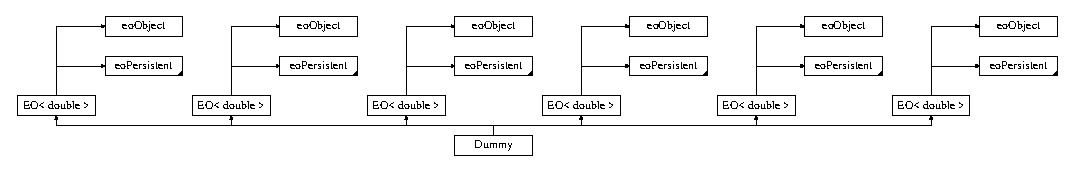
\includegraphics[height=1.86667cm]{struct_dummy}
\end{center}
\end{figure}
\subsection*{Public Types}
\begin{CompactItemize}
\item 
typedef double {\bf Type}\label{struct_dummy_w0}

\item 
typedef double {\bf Type}\label{struct_dummy_w1}

\item 
typedef double {\bf Type}\label{struct_dummy_w2}

\item 
typedef double {\bf Type}\label{struct_dummy_w3}

\item 
typedef double {\bf Type}\label{struct_dummy_w4}

\item 
typedef double {\bf Type}\label{struct_dummy_w5}

\end{CompactItemize}
\subsection*{Public Member Functions}
\begin{CompactItemize}
\item 
{\bf Dummy} (std::string \_\-s=\char`\"{}\char`\"{})\label{struct_dummy_a0}

\item 
void {\bf print\-On} (std::ostream \&\_\-os) const 
\begin{CompactList}\small\item\em Write object. \item\end{CompactList}\item 
void {\bf print\-On} (std::ostream \&\_\-os) const 
\begin{CompactList}\small\item\em Write object. \item\end{CompactList}\item 
void {\bf print\-On} (std::ostream \&\_\-os) const 
\begin{CompactList}\small\item\em Write object. \item\end{CompactList}\item 
void {\bf print\-On} (std::ostream \&\_\-os) const 
\begin{CompactList}\small\item\em Write object. \item\end{CompactList}\end{CompactItemize}
\subsection*{Public Attributes}
\begin{CompactItemize}
\item 
std::string {\bf s}\label{struct_dummy_o0}

\item 
double {\bf xdist}\label{struct_dummy_o1}

\end{CompactItemize}


\subsection{Detailed Description}
test program for the general operator - millenium version! uses dummy individuals 



Definition at line 27 of file t-eo\-Checkpointing.cpp.

\subsection{Member Function Documentation}
\index{Dummy@{Dummy}!printOn@{printOn}}
\index{printOn@{printOn}!Dummy@{Dummy}}
\subsubsection{\setlength{\rightskip}{0pt plus 5cm}void Dummy::print\-On (std::ostream \& {\em \_\-os}) const\hspace{0.3cm}{\tt  [inline, virtual]}}\label{struct_dummy_a1}


Write object. 

Called print\-On since it prints the object \_\-on\_\- a stream. \begin{Desc}
\item[Parameters:]
\begin{description}
\item[{\em \_\-os}]A std::ostream. \end{description}
\end{Desc}


Reimplemented from {\bf EO$<$ double $>$} {\rm (p.\,\pageref{class_e_o_z10_2})}.

Definition at line 41 of file t-eo\-Gen\-Op.cpp.

References EO$<$ F $>$::print\-On().\index{Dummy@{Dummy}!printOn@{printOn}}
\index{printOn@{printOn}!Dummy@{Dummy}}
\subsubsection{\setlength{\rightskip}{0pt plus 5cm}void Dummy::print\-On (std::ostream \& {\em \_\-os}) const\hspace{0.3cm}{\tt  [inline, virtual]}}\label{struct_dummy_a2}


Write object. 

Called print\-On since it prints the object \_\-on\_\- a stream. \begin{Desc}
\item[Parameters:]
\begin{description}
\item[{\em \_\-os}]A std::ostream. \end{description}
\end{Desc}


Reimplemented from {\bf EO$<$ double $>$} {\rm (p.\,\pageref{class_e_o_z10_2})}.

Definition at line 23 of file t-eo\-Replacement.cpp.

References EO$<$ F $>$::print\-On().\index{Dummy@{Dummy}!printOn@{printOn}}
\index{printOn@{printOn}!Dummy@{Dummy}}
\subsubsection{\setlength{\rightskip}{0pt plus 5cm}void Dummy::print\-On (std::ostream \& {\em \_\-os}) const\hspace{0.3cm}{\tt  [inline, virtual]}}\label{struct_dummy_a3}


Write object. 

Called print\-On since it prints the object \_\-on\_\- a stream. \begin{Desc}
\item[Parameters:]
\begin{description}
\item[{\em \_\-os}]A std::ostream. \end{description}
\end{Desc}


Reimplemented from {\bf EO$<$ double $>$} {\rm (p.\,\pageref{class_e_o_z10_2})}.

Definition at line 18 of file t-eo\-Select.cpp.

References EO$<$ F $>$::print\-On().\index{Dummy@{Dummy}!printOn@{printOn}}
\index{printOn@{printOn}!Dummy@{Dummy}}
\subsubsection{\setlength{\rightskip}{0pt plus 5cm}void Dummy::print\-On (std::ostream \& {\em \_\-os}) const\hspace{0.3cm}{\tt  [inline, virtual]}}\label{struct_dummy_a4}


Write object. 

Called print\-On since it prints the object \_\-on\_\- a stream. \begin{Desc}
\item[Parameters:]
\begin{description}
\item[{\em \_\-os}]A std::ostream. \end{description}
\end{Desc}


Reimplemented from {\bf EO$<$ double $>$} {\rm (p.\,\pageref{class_e_o_z10_2})}.

Definition at line 24 of file t-eo\-Sharing.cpp.

References EO$<$ F $>$::print\-On().

The documentation for this struct was generated from the following files:\begin{CompactItemize}
\item 
t-eo\-Checkpointing.cpp\item 
t-eo\-Gen\-Op.cpp\item 
t-eo\-Replacement.cpp\item 
t-eo\-Select.cpp\item 
t-eo\-Sharing.cpp\item 
t-eo\-State\-And\-Parser.cpp\end{CompactItemize}
